\chapter{Introduzione}
\label{cap:introduzione}

\begin{figure}[h!]
    \centering
    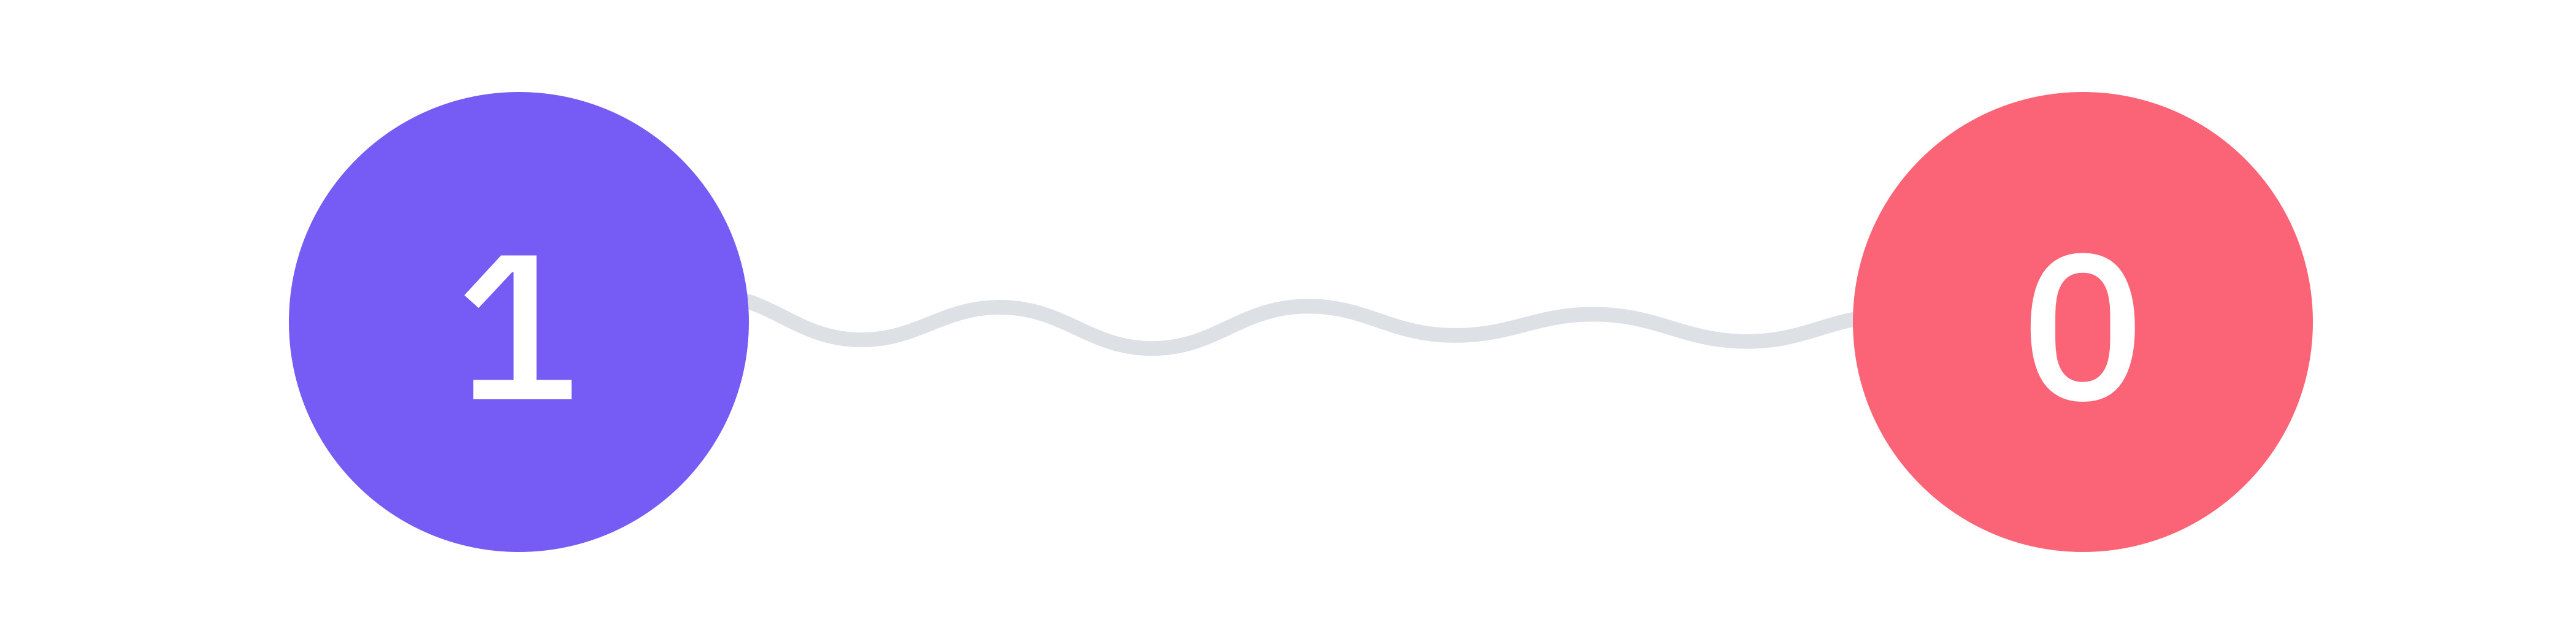
\includegraphics[width=1\columnwidth]{img/quantum_entanglement.jpeg}
    \caption{Lorem}
    \label{fig:entanglement}
\end{figure}

Introduzione al contesto applicativo.

Lorem Figure \ref{fig:entanglement}

Esempio di utilizzo di un termine nel glossario \gls{api}.

Esempio di citazione in linea
\cite{site:agile-manifesto}.

Esempio di citazione nel pie' di pagina
citazione\footcite{womak:lean-thinking}

Termine di glossario \gls{apig}

\lipsum[1-2]

\section{L'azienda}

\lipsum[1]

\section{L'idea}

Introduzione all'idea dello stage\footcite{article:spooky}.
\lipsum[1-3]

\section{Organizzazione del testo}

\begin{description}
    \item[{\hyperref[cap:processi-metodologie]{Il secondo capitolo}}] descrive ...
    
    \item[{\hyperref[cap:descrizione-stage]{Il terzo capitolo}}] approfondisce ...
    
    \item[{\hyperref[cap:analisi-requisiti]{Il quarto capitolo}}] approfondisce ...
    
    \item[{\hyperref[cap:progettazione-codifica]{Il quinto capitolo}}] approfondisce ...
    
    \item[{\hyperref[cap:verifica-validazione]{Il sesto capitolo}}] approfondisce ...
    
    \item[{\hyperref[cap:conclusioni]{Nel settimo capitolo}}] descrive ...
\end{description}

Riguardo la stesura del testo, relativamente al documento sono state adottate le seguenti convenzioni tipografiche:
\begin{itemize}
	\item gli acronimi, le abbreviazioni e i termini ambigui o di uso non comune menzionati vengono definiti nel glossario, situato alla fine del presente documento;
	%\item per la prima occorrenza dei termini riportati nel glossario viene utilizzata la seguente nomenclatura: \emph{parola}\glsfirstoccur;
	\item i termini in lingua straniera o facenti parti del gergo tecnico sono evidenziati con il carattere \emph{corsivo}.
\end{itemize}
